\documentclass[a4paper,12pt]{article}
\usepackage[swedish]{babel}
\usepackage[utf8]{inputenc}
\usepackage{amsmath, amsthm, amssymb}
\usepackage{pgfplots, scrextend}
\pgfplotsset{compat=1.18}
% Ändra INTE nästa rad (säger var texten ska typsättas)
\usepackage[a4paper,includeheadfoot,margin=2.54cm]{geometry}
% Ändra INTE nästa rad (som lägger till radnummer till vänster)
\usepackage[left]{lineno}


% Ändra INTE raderna nedan
% Koden är från https://tex.stackexchange.com/questions/43648/
% Den fixar radnumrering av text i närvaro av matematikomgivningar
\newcommand*\patchAmsMathEnvironmentForLineno[1]{%
  \expandafter\let\csname old#1\expandafter\endcsname\csname #1\endcsname
  \expandafter\let\csname oldend#1\expandafter\endcsname\csname end#1\endcsname
  \renewenvironment{#1}%
     {\linenomath\csname old#1\endcsname}%
     {\csname oldend#1\endcsname\endlinenomath}}% 
\newcommand*\patchBothAmsMathEnvironmentsForLineno[1]{%
  \patchAmsMathEnvironmentForLineno{#1}%
  \patchAmsMathEnvironmentForLineno{#1*}}%
\AtBeginDocument{%
\patchBothAmsMathEnvironmentsForLineno{equation}%
\patchBothAmsMathEnvironmentsForLineno{align}%
\patchBothAmsMathEnvironmentsForLineno{flalign}%
\patchBothAmsMathEnvironmentsForLineno{alignat}%
\patchBothAmsMathEnvironmentsForLineno{gather}%
\patchBothAmsMathEnvironmentsForLineno{multline}%
}

% Ändra INTE nästa rad (gör så radnummer skrivs med fet stil)
\renewcommand\linenumberfont{\normalfont\bfseries\small}

\title{Skidbacken}
%
\author{Zacharias Brohn\thanks{email:
        \texttt{zacbro-8@student.ltu.se}}\\  
        ~ \\
        Luleå tekniska universitet \\ 
        971 87 Luleå, Sverige}
%          
\date{\today}

\begin{document}

\linenumbers % ger radnumrering

\maketitle

\begin{abstract}
  Denna rapport handlar om LoremIpsum
  Denna rapport handlar om LoremIpsum  Denna rapport handlar om LoremIpsum  Denna rapport handlar om LoremIpsum  Denna rapport handlar om LoremIpsum  Denna rapport handlar om LoremIpsum  Denna rapport handlar om LoremIpsum  Denna rapport handlar om LoremIpsum  Denna rapport handlar om LoremIpsum  Denna rapport handlar om LoremIpsum  Denna rapport handlar om LoremIpsum  Denna rapport handlar om LoremIpsum  Denna rapport handlar om LoremIpsum  Denna rapport handlar om LoremIpsum  Denna rapport handlar om LoremIpsum  Denna rapport handlar om LoremIpsum  Denna rapport handlar om LoremIpsum  Denna rapport handlar om LoremIpsumDenna rapport handlar om LoremIpsum  Denna rapport handlar om LoremIpsum  Denna rapport handlar om LoremIpsum  Denna rapport handlar om LoremIpsum  Denna rapport handlar om LoremIpsum  Denna rapport handlar om LoremIpsum  Denna rapport handlar om LoremIpsum  Denna rapport handlar om LoremIpsum  Denna rapport handlar om LoremIpsum  Denna rapport handlar om LoremIpsum  Denna rapport handlar om LoremIpsum  Denna rapport handlar om LoremIpsumDenna rapport handlar om LoremIpsum  Denna rapport handlar om LoremIpsum  Denna rapport handlar om LoremIpsum  Denna rapport handlar om LoremIpsum  Denna rapport handlar om LoremIpsum  Denna rapport handlar om LoremIpsum  Denna rapport handlar om LoremIpsum  Denna rapport handlar om LoremIpsum  Denna rapport handlar om LoremIpsum  Denna rapport handlar om LoremIpsum  Denna rapport handlar om LoremIpsum  Denna rapport handlar om LoremIpsumDenna rapport handlar om LoremIpsum  Denna rapport handlar om LoremIpsum  Denna rapport handlar om LoremIpsum  Denna rapport handlar om LoremIpsum  Denna rapport handlar om LoremIpsum  Denna rapport handlar om LoremIpsum  Denna rapport handlar om LoremIpsum  Denna rapport handlar om LoremIpsum  Denna rapport handlar om LoremIpsum  Denna rapport handlar om LoremIpsum  Denna rapport handlar om LoremIpsum  Denna rapport handlar om LoremIpsum
\end{abstract}
\section{Introduktion}
\label{sec:introduktion}
Rapporten kommer lösa och beskriva uppgifter kring en skidbacke som har fallhöjden 500 meter. Här ser du den grafiskt ritad:

\noindent
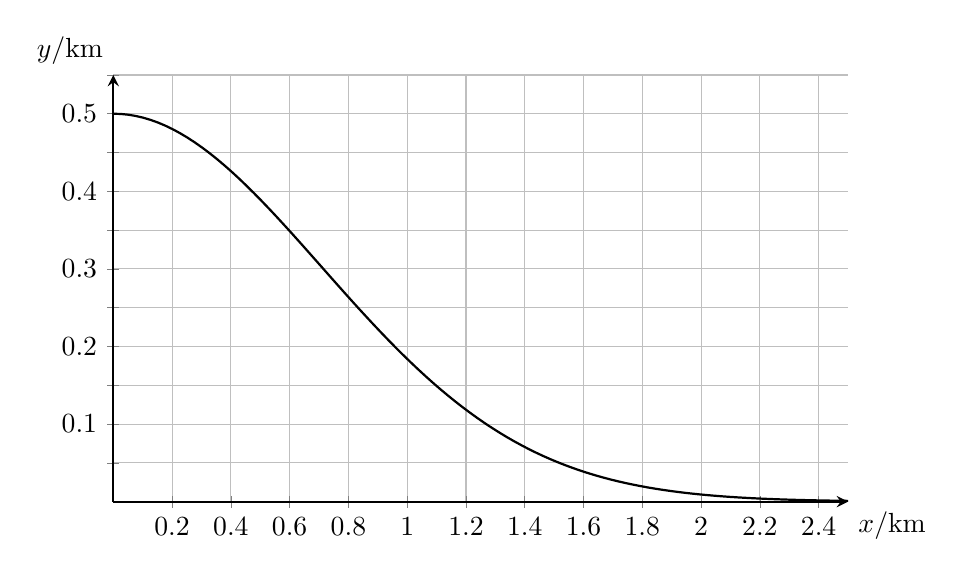
\begin{tikzpicture}
  \begin{axis}[
      width=0.9\linewidth,
      height=7cm,
      %axis tick,  % Equal scaling on both axes
      axis lines=middle, % Draw the axes in the middle with arrows
      xlabel={$x$/km},
      ylabel={$y$/km},
      domain=0:2.5,      % Set the range for x-axis
      samples=100,       % Set the number of samples for smoothness
      xmin=0,            % Start x-axis from 0
      ymin=0,            % Start y-axis from 0
      xmax=2.5,          % Limit x-axis to 2.5 for matching graph
      ymax=0.55,          % Limit y-axis to 0.5
      grid=major,        % Major grid only
      thick,             % Thicker lines
      every axis x label/.style={at={(current axis.right of origin)}, anchor=north west},
      every  axis y label/.style={at={(current axis.above origin)}, anchor=south east},
      xtick={0,0.2,...,2.5},  % Define x-tick steps
      ytick={0,0.05,0.1,...,0.6},  % Define y-tick steps
      yticklabels={0.0,,0.1,,0.2,,0.3,,0.4,,0.5,,0.6}
  ]
      \addplot[black] {0.5*exp(-x^2)};
  \end{axis}
\end{tikzpicture}\newline
Grafen är ritad med ett samband mellan y (höjden i km.) och x (längden i km.) som kan srivas som:\\
$y = 0,5e^{-x^2}$ $\>$ $\>$ där $\>$ $\>$ $0 \leq x \leq 2,5$\\
\section{En skidbackes lutning}
\label{sec:uppg1}
  Först löser vi uppgiften:\\
  \begin{addmargin}[1em]{1em}
    Bestäm backens lutning för $x = 0,8$.\\
  \end{addmargin}
  För att räkna fram lutningen måste vi lista ut och använda funktionens derivata $f'(x)$. Genom att använda kedjeregeln $(f(g(x)) = f'(g(x))g'(x))$ så får vi
  \begin{equation}
    \frac{d}{dx}\left(e^{-x^2}\right) = \frac{d}{dx}e^4\frac{du}{dx},
  \end{equation}
  där
  \begin{displaymath}
    u = -x^2
  \end{displaymath}
  och
  \begin{displaymath}
    \frac{d}{du}\left(e^4\right) = e^u
  \end{displaymath}
  och där
  \begin{displaymath}
    \frac{d}{dx}\left(-x^2\right) = -2x \text{ ty,} \frac{d}{dx} = n \cdot x^{n-1}.
  \end{displaymath}
  vilket ger oss
  \begin{displaymath}
    -0,5\left(\frac{2x}{e^{x^2}}\right) = \frac{-x}{e^{x^2}} = -x \cdot e^{-x^2}.
  \end{displaymath}
\section{Nästa (del-) uppgift}
\label{sec:uppg2}

\section{Och ännu nästa (del-) uppgift...}
\label{sec:uppgN}

\section{Diskussion [och slutsatser]}
\label{sec:disk}

Sammanfatta vad som avhandlats i rapporten, vad du kommit fram till,
och sätt det i sitt sammanhang. 
%
\begin{thebibliography}{99}
%
\bibitem{latexcompanion} 
Michel Goossens, Frank Mittelbach, and Alexander Samarin. 
\textit{The \LaTeX\ Companion}. 
Addison-Wesley, Reading, Massachusetts, 1993.
%
\bibitem{einstein} 
Albert Einstein. 
\textit{Zur Elektrodynamik bewegter K{\"o}rper}. (German) 
[\textit{On the electrodynamics of moving bodies}]. 
Annalen der Physik, 322(10):891–921, 1905.
%
\end{thebibliography}
%
\end{document}
